\documentclass{article}%
\usepackage[T1]{fontenc}%
\usepackage[utf8]{inputenc}%
\usepackage{lmodern}%
\usepackage{textcomp}%
\usepackage{lastpage}%
\usepackage{authblk}%
\usepackage{graphicx}%
%
\title{Magnesium Lithospermate B, an Active Extract of Salvia miltiorrhiza, Mediates sGC/cGMP/PKG Translocation in Experimental Vasospasm}%
\author{Dana Sandoval}%
\affil{Priority Research Centre for Cancer Research, University of Newcastle, Callaghan, NSW, Australia}%
\date{01{-}01{-}2009}%
%
\begin{document}%
\normalsize%
\maketitle%
\section{Abstract}%
\label{sec:Abstract}%
A team of scientists at the University of Hawaii and California Polytechnic State University, Polytechnic (Cal State San Luis Obispo), recently identified a pollen self{-}incompatibility determinant in Papaver rhoeas. The finding could help advance efforts to develop developing a cure for depression, anxiety and other psychiatric illnesses.\newline%
The researchers identified a self{-}incompatibility determinant of papaver rhoeas that has independently evolved in both North American and European mammals in the post{-}humans period to improve the immune system. The findings are published online by The New England Journal of Medicine.\newline%
The cooperative research team headed by Monica Yamada, Ph.D., associate professor in the Department of Molecular Sciences in the College of Biological Sciences at Cal State San Luis Obispo, and Travis Gray, Ph.D., distinguished professor in the Division of Developmental Biology at Cal Poly, were able to identify this pollen self{-}incompatibility determinant based on unique characteristics in the nine species of papaver rhoea.\newline%
We were able to identify this self{-}incompatibility determinant of papaver rhoea given two needs, said Yamada. First, the critical benefit is superior immunity to microbial and local microbial pathogens, including viruses and bacteria, which can include listeria, to virus and bacteria.\newline%
The second issue is lack of a lipid lactidase{-}1 (LLAR1) lignin, an important indicator of eczema and allergic reactions, specifically those associated with female Papaver rhoea, who is susceptible to bacterial or human infection. Since pluripotent stem cells commonly have the benefit of the LLAR1 pathway in other tissues such as the brain, rodent and host tissues, it would provide additional clue as to how the immune system responds.\newline%
The researchers say this discovery could contribute to our understanding of why Papaver rhoea might have a better immune response to bacteria and viruses. Their next steps are to consider the biology of this novel self{-}incompatibility determinant.\newline%
This study is a scientific benchmark because it gives us the first biological indication of self{-}incompatibility in Papaver rhoea, said Gray. We are already going into the neophyte of the field to make sure the results are credible.

%
\subsection{Image Analysis}%
\label{subsec:ImageAnalysis}%


\begin{figure}[h!]%
\centering%
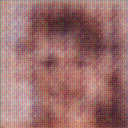
\includegraphics[width=150px]{500_fake_images/samples_5_265.png}%
\caption{A Close Up Of A Small Black And White Cat}%
\end{figure}

%
\end{document}